\section{Data Visualization}

\begin{frame}{Data Visualization}
	\textbf{Why visualize data?}
	\begin{itemize}
		\item \textbf{Gain insight} into an information space by mapping data into graphical primitives.
		\item \textbf{Provide qualitative overview} of large data sets.
		\item \textbf{Search} for patterns, trends, structure, irregularities, relationships among data.
		\item \textbf{Help find interesting regions and suitable parameters} for further quantitative analysis.
		\item \textbf{Provide a visual proof} of computer representations derived.
	\end{itemize}
	\textbf{Categorization of visualization methods:}
	\begin{itemize}
		\item Pixel-oriented.
		\item Geometric projection.
		\item Icon-based.
		\item Hierarchical.
		\item Visualizing complex data and relations.
	\end{itemize}
\end{frame}

\begin{frame}{Pixel Oriented Visualization Techniques}
	\begin{itemize}
		\item For a data set of $m$ dimensions create $m$ windows on the screen, one for each dimension.
		\item The values in dimension $m$ of a record are mapped to $m$ pixels at the corresponding \\ positions in the windows.
		\item The colors of the pixels reflect the corresponding values.
	\end{itemize}
	\vspace{0.5cm}
	\centering
	\includegraphics[width=9cm]{img/pixel.jpg}\\
	a) Income. \hspace{0.3cm} b) Credit limit. \hspace{0.2cm} c) Transaction volume. \hspace{0.2cm} (d) Age.
\end{frame}

\begin{frame}{Laying Out Pixels in a Spiderweb Diagram}
	To save space and show the connections among multiple dimensions, \\
	space filling is often done in a spiderweb diagram.\\
	\centering
	\begin{tikzpicture}[scale=0.8]
		\pie[hide number]{17/Dim 1, 17/Dim 2, 17/Dim 3, 17/Dim 4, 17/Dim 5, 16/Dim 6}
		\node at (1.5, 1) (a) {\tikzmark{t1} $\circ$};
		\node at (-1.5, 1) (b) {\tikzmark{t2} $\circ$};
		\node at (1.5, -0.9) (c) {\tikzmark{t3} $\circ$};
		\node at (-1.5, -0.9) (d) {\tikzmark{t4} $\circ$};
		\node at (0.1, -1.8) (e) {\tikzmark{t5} $\circ$};
		\node at (0, 1.8) (f) {\tikzmark{t6}$\circ$};
		\node at (-3, 3) (f) {Data record \tikzmark{n1}};
	\end{tikzpicture}
	\begin{tikzpicture}[remember picture,overlay]
		\path[draw=black,thick,-]<1-> (n1) -- (t1);
		\path[draw=black,thick,-]<1-> (n1) -- (t2);
		\path[draw=black,thick,-]<1-> (n1) -- (t3);
		\path[draw=black,thick,-]<1-> (n1) -- (t4);
		\path[draw=black,thick,-]<1-> (n1) -- (t5);
		\path[draw=black,thick,-]<1-> (n1) -- (t6);
	\end{tikzpicture}
\end{frame}

\begin{frame}{Laying Out Pixels in Circle Segments}
	To save space and show the connections among multiple dimensions, \\
	space filling is often done in a circle segment.\\
	\centering
	\newcommand{\D}{7} % number of dimensions (config option)
	\newcommand{\U}{7} % number of scale units (config option)

	\newdimen\R % maximal diagram radius (config option)
	\R=3.5cm
	\newdimen\L % radius to put dimension labels (config option)
	\L=4cm
	\newcommand{\A}{360/\D} % calculated angle between dimension axes

	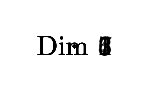
\begin{tikzpicture}[scale=0.7]
		\path (0:0cm) coordinate (O); % define coordinate for origin

		% draw the spiderweb
		\foreach \X in {1,...,\D}{
				\draw (\X*\A:0) -- (\X*\A:\R);
			}

		\foreach \Y in {0,...,\U}{
				\foreach \X in {1,...,\D}{
						\path (\X*\A:\Y*\R/\U) coordinate (D\X-\Y);
						\fill (D\X-\Y) circle (1pt);
					}
				\draw [opacity=0.3] (0:\Y*\R/\U) \foreach \X in {1,...,\D}{
						-- (\X*\A:\Y*\R/\U)
					} -- cycle;
			}

		% define labels for each dimension axis (names config option)
		\path (1*\A:\L) node (L1) {Dim 1};
		\path (2*\A:\L) node (L2) {Dim 2};
		\path (3*\A:\L) node (L3) {Dim 3};
		\path (4*\A:\L) node (L4) {Dim 4};
		\path (5*\A:\L) node (L5) {Dim 5};
		\path (6*\A:\L) node (L6) {Dim 6};
		\path (7*\A:\L) node (L7) {Dim 7};

		% for each sample case draw a path around the web along concrete values
		% for the individual dimensions. Each node along the path is labeled
		% with an identifier using the following scheme:
		%
		% D<d>-<v>, dimension <d> a number between 1 and \D (#dimensions) and
		% value <v> a number between 0 and \U (#scale units)
		%
		% The paths will be drawn half-opaque, so that overlapping parts will be
		% rendered in a composite color.

		% Example Case 1 (red)
		%
		% D1 (Security): 0/7; D2 (Content Quality): 5/7; D3 (Performance): 0/7;
		% D4 (Stability): 6/7; D5 (Usability): 0/7; D6 (Generality): 5/7;
		% D7 (Popularity): 0/7
		\draw [color=red,line width=1.5pt,opacity=0.5]
		(D1-0) --
		(D2-5) --
		(D3-0) --
		(D4-6) --
		(D5-0) --
		(D6-5) --
		(D7-0) -- cycle;

		% Example Case 2 (green)
		%
		% D1 (Security): 2/7; D2 (Content Quality): 2/7; D3 (Performance): 5/7;
		% D4 (Stability): 1/7; D5 (Usability): 4/7; D6 (Generality): 1/7;
		% D7 (Popularity): 7/7
		\draw [color=green,line width=1.5pt,opacity=0.5]
		(D1-2) --
		(D2-2) --
		(D3-5) --
		(D4-1) --
		(D5-4) --
		(D6-1) --
		(D7-7) -- cycle;

		% Example Case 3 (blue)
		%
		% D1 (Security): 1/7; D2 (Content Quality): 7/7; D3 (Performance): 4/7;
		% D4 (Stability): 4/7; D5 (Usability): 3/7; D6 (Generality): 5/7;
		% D7 (Popularity): 2/7
		\draw [color=blue,line width=1.5pt,opacity=0.5]
		(D1-1) --
		(D2-7) --
		(D3-4) --
		(D4-4) --
		(D5-3) --
		(D6-5) --
		(D7-2) -- cycle;

	\end{tikzpicture}
\end{frame}

\begin{frame}{Geometric Projection Visualization Techniques}
	\begin{itemize}
		\item Visualization of geometric transformations and projections of data.
		\item \textbf{Methods}:
		      \begin{itemize}
			      \item Scatter plot and scatter plot matrices.
			      \item Landscapes.
			      \item Projection pursuit technique: \emph{Help users find meaningful projections of multidimensional data.}
			      \item Prosection views.
			      \item Hyperslice.
			      \item Parallel coordinates.
		      \end{itemize}
	\end{itemize}
\end{frame}

\begin{frame}{Scatter Plot Matrices}
	\centering
	\includegraphics[height=6.5cm]{img/scatterplot_matrix.pdf}
\end{frame}

\begin{frame}{Parallel Coordinate Plot}
	\centering
	\vspace{0.5cm}
	\begin{tikzpicture}
		\begin{groupplot}[
				group style={
						group name=iris,
						group size=4 by 1,
						horizontal sep=2cm
					},
				axis y line=left,
				hide x axis,
				width=2cm,
				height=6cm,
				xmin=0,
				xmax=0.5,
				enlarge y limits,
				every axis plot/.append style={opacity=0}
			]

			\nextgroupplot

			\pgfplotsinvokeforeach{0,...,\NumRows} % loop over all rows in table
			{
				% get value in sw column
				\pgfplotstablegetelem{####1}{sw}\of{\iris}%
				% add a coordinate at x=0 and that y-value
				\edef\temp{\noexpand\addplot coordinates {(0,\pgfplotsretval)} coordinate (sl####1);}
				\temp
			}

			\nextgroupplot

			\pgfplotsinvokeforeach{0,...,\NumRows}
			{
				\pgfplotstablegetelem{####1}{sl}\of{\iris}%
				\edef\temp{\noexpand\addplot coordinates {(0,\pgfplotsretval)} coordinate (sw####1);}
				\temp
			}

			\nextgroupplot

			\pgfplotsinvokeforeach{0,...,\NumRows}
			{
				\pgfplotstablegetelem{####1}{pw}\of{\iris}%
				\edef\temp{\noexpand\addplot coordinates {(0,\pgfplotsretval)} coordinate (pl####1);}
				\temp
			}

			\nextgroupplot

			\pgfplotsinvokeforeach{0,...,\NumRows}
			{
				\pgfplotstablegetelem{####1}{pl}\of{\iris}%
				\edef\temp{\noexpand\addplot coordinates {(0,\pgfplotsretval)} coordinate (pw####1);}
				\temp
			}

		\end{groupplot}

		% add labels below
		\foreach \i/\txt in {1/SW,2/SL,3/PW,4/PL}
		\node [below] at (iris c\i r1.south west) {\txt};


		% draw the lines
		% this dataset has three groups of fifty rows each, hence the start/stop values
		\foreach[
			evaluate=\j as \START using int(\j*50),
			evaluate=\j as \STOP using int((\j+1)*50-1),
		] \j/\clr in {0/blue,1/red,2/green}
			{
				\foreach \i in {\START,...,\STOP}
				\draw [color=\clr,opacity=0.5] (sl\i) -- (sw\i) -- (pl\i) -- (pw\i);
			}

	\end{tikzpicture}
\end{frame}

\begin{frame}{Icon Based Visualization}
	\centering
	\begin{itemize}
		\item \textbf{Visualization of the data values as features of icons.}
		\item \textbf{Typical visualization methods:}
		      \begin{itemize}
			      \item Chernoff faces.
			      \item Stick figures.
		      \end{itemize}
		\item \textbf{General techniques:}
		      \begin{itemize}
			      \item Shape coding: \emph{Use shape to represent certain information encoding.}
			      \item Color icons: \emph{Use color icons to encode more information.}
			      \item Tile bars: \emph{Use small icons to represent the relevant feature vectors in document retrieval.}
		      \end{itemize}
	\end{itemize}
\end{frame}

\begin{frame}{Chernoff Faces}
	\textbf{A way to display variables on a two-dimensional surface:}\\
	E.g. let $x$ be eyebrow slant, $y$ be eye size, $z$ be nose length etc.\\
	The figure shows faces produced using $10$ characteristics (head eccentricity, eye size, eye spacing, eye eccentricity, pupil size, eyebrow slant, nose size, mouth shape, mouth size, and mouth opening). Each assigned one of $10$ possible values, generated using \href{https://www.wolfram.com/mathematica/}{Mathematica} (S. Dickson).\\[0.5cm]
	\centering
	\includegraphics[width=4cm]{img/chernoff_faces_construction.pdf}
\end{frame}

\begin{frame}{Stick Figure}
	A census data figure showing age, income, gender, education etc. \\
	A $5$-piece stick figure ($1$ body and $4$ limbs w. different angle/length).\\[0.1cm]
	\centering
	\includegraphics[width=8cm, height=5.2cm]{img/stick_figure.png}\\
	\tiny{Used by permission of G. Grinstein, University of Massachusettes at Lowell.}
\end{frame}

\begin{frame}{Hierarchical Visualization Techniques}
	\centering
	\begin{itemize}
		\item \textbf{Visualization of the data using a hierarchical partitioning into subspaces.}
		\item \textbf{Methods:}
		      \begin{itemize}
			      \item Worlds within worlds.
			      \item Tree maps.
			      \item Cone trees.
			      \item Info cube.
		      \end{itemize}
	\end{itemize}
\end{frame}

\begin{frame}{Worlds Within World}
	\begin{itemize}
		\item Assign the function and two most important parameters to innermost world.
		\item Fix all other parameters at constant values -- draw other (1,2 or 3) dimensional worlds choosing these as the axes.
	\end{itemize}
	\centering
	\includegraphics[width=8cm,height=5.2cm]{img/www.jpg}
\end{frame}

\begin{frame}{Tree Maps}
	\centering
	\begin{itemize}
		\item \textbf{Screen filling method:}
		      \begin{itemize}
			      \item Uses a hierarchical partitioning of the screen into regions depending on the attribute values.
			      \item $x$ and $y$-coordinates of the screen partitioned alternately according to the attribute values.
		      \end{itemize}
	\end{itemize}
	\begin{tikzpicture}[xscale = 1.35, yscale = 0.77,
			font=\sffamily,
			mystyle/.style={draw=white, very thick, text=white, font=\sffamily\bfseries},
		]
		\pie[square,
			style={mystyle},
			color={yellow!80!orange, gray, blue!40, orange},
			text=legend,
		]{68/A, 5/B, 5/C, 22/D}
	\end{tikzpicture}
\end{frame}

\begin{frame}{Tree Map of a File System}
	\centering
	\vspace{0.5cm}
	\includegraphics[width=9cm, height=6cm]{img/treemap_filesystem.png}
\end{frame}

\begin{frame}{Info Cubes}
	\begin{itemize}
		\item $3$D visualization technique:
		      \begin{itemize}
			      \item Hierarchical information is displayed as nested semi-transparent cubes.
			      \item The outermost cubes correspond to the top level data, while the subnodes or the lower level data are represented as smaller cubes inside the outermost cubes, and so on.
		      \end{itemize}
	\end{itemize}
	\vspace{0.2cm}
	\centering
	\includegraphics[width=4cm,height=4cm]{img/infocube.png}
\end{frame}

\begin{frame}{Three Dimensional Cone Trees}
	\centering
	\begin{itemize}
		\item $3$D cone-tree visualization technique:\\
		      works well for up to approx. a thousand nodes.
		\item Build a $2$D circle tree that arranges its nodes in concentric circles centered on the root node.
		\item Overlaps can't be avoided projecting onto $2$D.
		\item G. Robertson, J. Mackinlay, S. Card. "Cone Trees: Animated 3D Visualizations of Hierarchical Information", ACM SIGCHI'91.
	\end{itemize}
	\vspace{0.2cm}
	\includegraphics[width=3cm,height=3cm]{img/threedcone_one.jpg}\hspace{1cm}
	\includegraphics[width=3cm,height=3cm]{img/threedcone_two.jpg}\\
	\tiny{Acknowledgement: \href{ttp://nadeausoftware.com/articles/visualization}{http://nadeausoftware.com/articles/visualization}.}
\end{frame}

\begin{frame}{Visualizing Complex Data and Relations}
	\centering
	\begin{itemize}
		\item \textbf{Visualizing non-numerical data: text and social networks.}
		\item \textbf{Tag cloud: visualizing user-generated tags.}
		      \begin{itemize}
			      \item The importance of tag is represented by font size/color.
			      \item Besides text data, there are also methods to visualize relationships, \\ such as visualizing social networks.
		      \end{itemize}
	\end{itemize}
	\includegraphics[width=7cm,height=4cm]{img/google_news.png}
\end{frame}
